\section{Related work}\label{sec:related-work}

\subsection{Economic modeling}\label{subsec:economic-modeling}
Until the late 1970s, modeling in economics consisted mostly of seperated macro-, microeconomic models.

Models of this kind are described as follows ~\cite{morgan2012models}:
\begin{enumerate}
  \item Micro-economic theory, i.e.\ the study of how firms and households make decisions\footnote{\url{www.aier.org/article/the-difference-between-micro-and-macro-economics/}}, uses sophisticated mathematical methods in modeling economic phenomena.
  \item Macroeconomics, i.e.\ the study of the economy as a whole\footnotemark[\value{footnote}] (aggregates), relies more on purpose-built models, often devised for policy advice.
\end{enumerate}

In the 1976, Robert E. Lucas Jr~\cite{lucas1976econometric} wrote an article stating that while some macroeconomic models are good for forcasting
they are not always suitable for evaluating policies.
Changes in policies may lead to a false evaluation because individual agents may adjust their behavior not anticipated in the model~\cite{HURTADO2014S12}.
This is knows as: Lucas critique.

This lead to the development of: Dynamic stochastic general equilibrium (DSGE) models, these models incorporated microeconomics into macroeconomics~\cite{moos2019facts}.
One key element of these models is the existence of stochastic parametric drift, i.e.\ stochastic drift is the change of the average value of a stochastic (random) process\footnote{\url{en.wikipedia.org/wiki/Stochastic_drift}}.
The randomness refers to the unexpected behavior of agents over time.

Other economists, think that the DSGE model is too restrictive.
The DSGE model assumes that an economy can reach and sustain an equilibrium.
Newer views state: economies are non-linear, complex dynamic systems, which rarely, if ever, reach an equilibrium~\cite{hamill2016agent}.
Because of this Agent base modeling is a way forward~\cite{hamill2016agent}.

The next citation from Howitt~\cite{howitt2012have} describes the compelling reason to use economic ABM as follows:

\textit{`Instead of assuming that people have an incredibly sophisticated ability to solve a computationally challenging intertemporal planning problem in an incredibly simple environment (the simplicity being needed in order to make the equilibrium computable), the ACE (i.e.
agent-based computational economics) approach is to assume that people have very simple rules of behavior for coping with an environment that is too complex for anyone fully to understand.'}

The survey conducted by Heath et al.~\cite{heath2009survey}, states that the complexity of systems also may be the cause of lacking meaningfully results emanating from ABM studies.
But they also state that there is no reason that they could not yield meaningfully results.
They say that special techniques, philosophies and methods need to be developed and to be taught.

\subsection{Agent Base Modeling}\label{subsec:agent-base-modeling}
The term Agent-Based Modeling (ABM) refers to a class of modeling methods designed for the study of systems whose dynamics are driven by successive interactions among heterogeneous entities~\cite{tesfatsion2023agent}.

Models of this kind simulate how artificial agents behave in an artificial environment over a time interval.
These agents can be anything e.g: ants , radioactive nuclei, viruses, as long as they have some properties that can change over time, and they respond to other agents and their environment.

Agents have the following properties~\cite{hamill2016agent}:
\begin{enumerate}
  \item Perception: agents can see other agents in their neighbourhood and their environment.
  \item Performance: agents can act, such as moving and communicating.
  \item Memory: agents can recall their past states and actions.
  \item Policy: agents can have rules that determine what they do next.
\end{enumerate}

The study from Heath et al.~\cite{heath2009survey} contains a simplified simulation (figure~\ref{fig:steps_simulation}) development process.

\begin{figure}
    \centering
    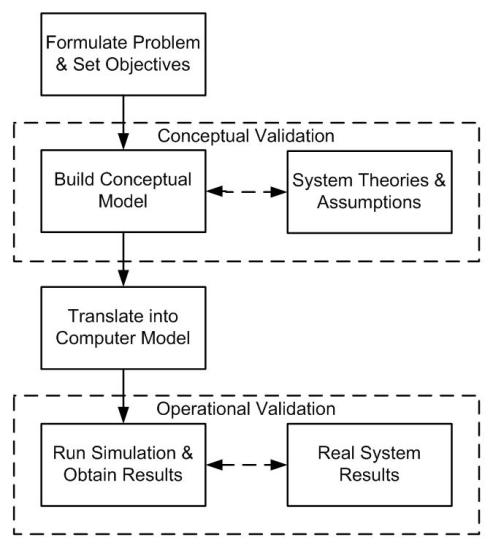
\includegraphics[width=8cm]{sections/pics/Steps_To_Build_Simulation}
    \caption{Similation Building Proces}
    \label{fig:steps_simulation}
\end{figure}

This process will be used for this study, except the validation with real system result.

Other research projects reported about the food delivery sector using the NetLogo tool.
An existing model for the food delivery context is created by~\cite{ismail2024software}.
This model was used to research the efficiency of food delivery.
The model consists riders, vendors and customers.
The world consists of a 2-dimensional grid where riders have to pick up food from vendors and deliver it to customers.
This project also mentioned some real world rules the 3 types of agents possess.

In another study ~\cite{antelmi2024reliable} NetLogo is compared to other ABM systems and integrations with other programming languages are analysed.



% Check this: ~\cite{cincotti2022we}


